\documentclass[12pt]{article}
%\usepackage{alltt}
%\usepackage{helvet}
%\usepackage[sfdefault]{roboto}
\usepackage{amsmath}
\usepackage[utf8]{inputenc}
\usepackage[dvips]{graphicx}
%\usepackage{a4wide}
\usepackage{epsfig}
\usepackage{fancybox}
\usepackage{verbatim}
\usepackage{array}
\usepackage{latexsym}
\usepackage{alltt}
\usepackage{url}
\usepackage{color}   % added for colored text
%\usepackage{fullpage}
\usepackage{hyperref}
\usepackage{listings}
\usepackage{color}
\usepackage{calc}
\usepackage{enumitem}
\usepackage[hmargin=3cm,vmargin=5.0cm]{geometry}
%\topmargin=0cm
\topmargin=-1.8cm \addtolength{\textheight}{4.5cm}
\addtolength{\textwidth}{1.0cm}
%\setlength{\leftmargin}{-5cm}
\setlength{\oddsidemargin}{0.0cm}
\setlength{\evensidemargin}{0.0cm}

%\renewcommand{\familydefault}{\sfdefault}

\newcommand{\HRule}{\rule{\linewidth}{1mm}}
\newcommand{\kutu}[2]{\framebox[#1mm]{\rule[-2mm]{0mm}{#2mm}}}
\newcommand{\gap}{ \\[1mm] }

\newcommand{\Q}{\raisebox{1.7pt}{$\scriptstyle\bigcirc$}}

\definecolor{amaranth}{rgb}{0.9, 0.17, 0.31}
\definecolor{gray}{rgb}{0.4,0.4,0.4}
\definecolor{darkblue}{rgb}{0.0,0.0,0.6}
\definecolor{cyan}{rgb}{0.0,0.6,0.6}
\definecolor{red}{rgb}{0.6,0,0}
\definecolor{dkgreen}{rgb}{0,0.6,0}
\definecolor{mauve}{rgb}{0.58,0,0.82}
\definecolor{lightblue}{rgb}{0.0,0.0,0.9}
\definecolor{darkred}{rgb}{0.6,0.0,0.0}

\lstset{
    %backgroundcolor=\color{lbcolor},
    tabsize=4,
    basicstyle=\fontsize{10}{10.3}\selectfont\sffamily,
    numberstyle=\footnotesize,
    aboveskip={0.0\baselineskip},
    belowskip={0.0\baselineskip},
    columns=fullflexible,
    breaklines=true,
    prebreak=\raisebox{0ex}[0ex][0ex]{\ensuremath{\hookleftarrow}},
    frame=single,
    showtabs=false,
    showspaces=false,
    showstringspaces=false,
    identifierstyle=\color{amaranth},
    keywordstyle=\color{rgb}{0,0,1},
    commentstyle=\color[rgb]{0.133,0.545,0.133},
    stringstyle=\color{amaranth},
}

\lstdefinelanguage{XML}
{
  morestring=[s][\color{red}]{"}{"},
  morestring=[s][\color{black}]{>}{<},
  morecomment=[s]{<?}{?>},
  morecomment=[s][\color{dkgreen}]{<!--}{-->},
  %stringstyle=\color{black},
  identifierstyle=\color{black},
  keywordstyle=\color{darkblue},
  commentstyle=\color[rgb]{0.133,0.545,0.133},
  stringstyle=\color{black},
  morekeywords={Scene,BackgroundColor,ShadowRayEpsilon,
  MaxRecursionDepth,Cameras,Camera,Position,Gaze,Up,
  NearPlane,NearDistance,ImageResolution,ImageName,
  Material,Materials,VertexData,Mesh,Triangle,Sphere,
  Faces,Lights,AmbientLight,PointLight,Objects,Indices,
  AmbientReflectance,DiffuseReflectance,SpecularReflectance,PhongExponent,MirrorReflectance,Intensity,Center,Radius,xmlns,version}% list your attributes here
}

\begin{document}

\noindent \HRule \\[3mm]
\small
\begin{tabular}[b]{lp{1.2cm}r}
\href{https://www.metu.edu.tr/}{
\epsfig{file=metulogo.eps,width=5mm}} Middle East Technical
University &  &
\href{https://ceng.metu.edu.tr/information}{
\epsfig{file=bmblogo.eps,width=5mm}} Department of Computer Engineering \\
\end{tabular} \\
\begin{center}

                 \LARGE \textbf{CENG 795} \\[4mm]
                 \Large Advanced Ray Tracing \\[4mm]
                \normalsize Fall '2022-2023 \\
                    \normalsize Assignment 4 - All About Textures \\
                    \normalsize (v.1.0)
\end{center}
\HRule

\begin{center}
Due date: December 15, 2022, Thursday, 23:59
\end{center}

\centerline{
    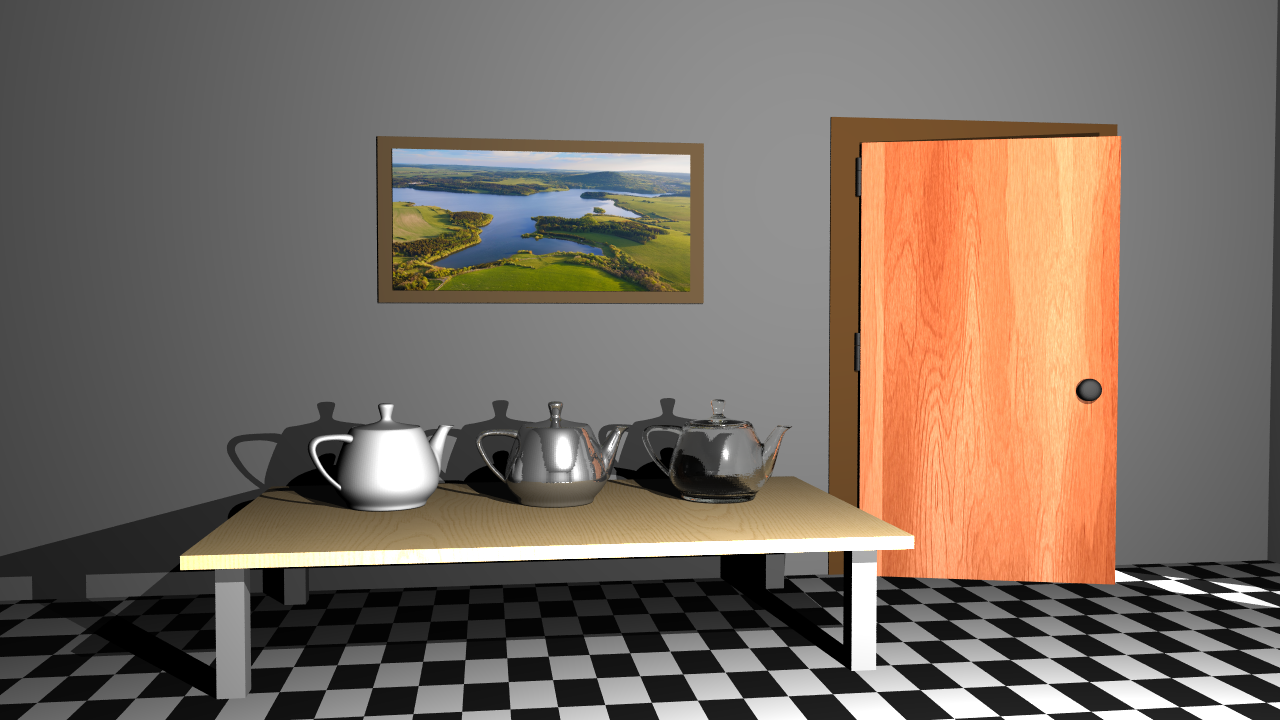
\includegraphics[width=5in]{../outputs/veach_ajar/VeachAjar.png}
}

\section{Objectives}

In this homework you are expected to add texture mapping capabilities to your ray
tracers. We will be using textures for five main purposes:

\begin{itemize}
    \item Background textures for rays not hitting any objects (replace\_background)
    \item Diffuse and specular reflectance maps (replace\_kd, blend\_kd, replace\_ks) for objects
    \item To disable shading and simply paste the texture color on an object (replace\_all)
    \item Normals maps (replace\_normal)
    \item Bump maps (bump\_normal)
\end{itemize}

We will be dealing with two types of textures:

\begin{itemize}
\item Image textures (typically PNG and JPEG files -- you can use any image reader library)
\item Perlin noise (generated for each point on the fly)
\end{itemize}

\vspace{0.5cm} \noindent \textbf{Keywords:} \emph{multisampling,
    aliasing, reconstruction, filtering, distribution ray tracing}

\section{Specifications}
\begin{enumerate}


\item \textbf{}The specifications are the same as for the previous
homeworks so are not repeated here. 

\end{enumerate}

\section{Scene File}
\label{sec:sceneFile}

\noindent Please see the previous assignments for a detailed
description of the scene file.  In this section, only the elements
introduced in this homework are explained.

\begin{itemize}

\item \textbf{Textures:} 

All of the specifications regarding texture mapping are defined under
this element. It contains two types of child elements: Images and
TextureMap. Images are simply a list of image files. An example is
below:

\begin{verbatim}
<Images>
    <Image id="1">textures/galaxy.jpg</Image>
    <Image id="2">textures/rap01.jpg</Image>
</Images>
\end{verbatim}

Separating images from texture maps allows one to use the same image
for different texture maps, avoiding memory duplication. For example,
one mesh can use an image with nearest-neighbor sampling and another
can use the same image with bilinear sampling.

TextureMaps define the properties of actual texture mapping. An
example is given below:

\begin{verbatim}
<TextureMap id="1" type="image">
    <ImageId>2</ImageId>
    <DecalMode>replace_kd</DecalMode>
    <Interpolation>bilinear</Interpolation>
</TextureMap>
\end{verbatim}

This defines that the texture map with id 1 is an image texture
according to its type attribute. The other two possible types are
\emph{perlin} and \emph{checkerboard}.  You can of course extend this
list, but these are the values we use for the homework.

\begin{itemize}
\item \textbf{ImageId:} an index into the images element. Only texture
maps whose type is \emph{image} use this element.

\item \textbf{DecalMode:} the mode of texture mapping. The possible
values are the following:

\begin{itemize}
\item replace\_kd: Use the texture value as $k_d$ value. Currently,
    divide the texture color value by $255$ to obtain a three channel
    $k_d$ value between $[0,1]$ for each component. Textures defined like this are called
    diffuse textures.
\item blend\_kd: Equally mix the existing material $k_d$ value with
the one that comes from the texture.
\item replace\_ks: Use the texture value as $k_s$ values. Currently,
    divide the texture color value by $255$ to obtain a three channel
    $k_s$ value between $[0,1]$ for each component. Textures defined like this are called
    specular textures.
\item replace\_background: This texture defines the background texture
    of the scene. You can think of this texture as the texture of the
    near plane. Only one texture can be defined as the background
    texture. If this texture is defined, the BackgroundColor element
    is ignored.
\item replace\_normal: Use this texture for normal mapping. Note that
    this texture is defined in the canonical tangent space and the
    normal vector that it defines must be transformed to the actual
    tangent space of the surface.
\item bump\_normal: Use this texture for bump mapping. 
\item replace\_all: Replace all components (i.e. diffuse, specular,
        and ambient) of the surface shading color with this texture's
     value.
\end{itemize}

\item \textbf{Interpolation:} Defines whether nearest or bilinear
interpolation should be used. If bilinear interpolation is defined
and you are fetching a texel value from an edge pixel, you can repeat
this edge pixel to avoid out-of-bounds access.

\item \textbf{BumpFactor:} In bump mapping, it may be desirable to
control the strength of the displacement function. This value
determines this multiplication factor. In other words, you must
multiply your displacement function with the value of this element to
compute the real displacement.

\item \textbf{NoiseScale:} This element only applies to Perlin noise
textures. It is used to control the frequency of the Perlin noise.
For implementation you must multiply the input position that you give
to the noise function with this value. Smaller scales will create a
low frequency noise texture and larger scales will create a high
frequency noise texture.

\item \textbf{NoiseScale:} This element only applies to Perlin noise
textures. It defines whether you should take the absolute value
(absval) of the noise function or whether you should linearly convert
it (linear) to $[0,1]$ range. If you take the absolute value, you get
the snake-like patterns. Otherwise, you get a more patch noisy result.

In addition to the image and Perlin textures, there is another procedural
texture called the \emph{checkerboard} texture that comes handy in
certain scenarios. For example, the ground plane in the Veach-Ajar
scene is defined using this texture. A checkerboard texture can be
created using the following pseudo-code:

\begin{verbatim}
bool x = (int) ((pos.x + offset) * scale) % 2; 
bool y = (int) ((pos.y + offset) * scale) % 2; 
bool z = (int) ((pos.z + offset) * scale) % 2;

bool xorXY = x != y;

if (xorXY != z) 
    return black; 
else 
    return white; 
\end{verbatim}

Here, the \texttt{pos} variable is the 3D point at which we are calculating the
texture value. \texttt{offset} controls the starting point of the
pattern. By changing the offset, you can shift the pattern in the 3D
space. \texttt{scale} controls the size of the checkerboard squares.
\texttt{black} and \texttt{white} define the colors of the checkerboard
squares -- they do not have to be black and white: you can define a
purple and orange checkerboard if it suits your taste. These parameters
are defined using the following XML elements:

\item \textbf{Scale:} the \texttt{scale} variable defined above
\item \textbf{Offset:} the \texttt{offset} variable defined above
\item \textbf{BlackColor:} a color triplet defines the color of the
``black'' squares
\item \textbf{WhiteColor:} a color triplet defines the color of the
``white'' squares

Up to know, we discussed the definition of textures. How can we
actually use them for texture mapping on meshes? All object types we
learned so far (Triangle, Sphere, Mesh, and MeshInstance) now also
accept a new element called \emph{Textures}. This element simply
defines which TextureMaps defined previously in the file should be
used for texture mapping on that object. Note that the Textures
element can contain multiple values. For example, if we want to define
a diffuse map, specular map, and a bump map for an object its
Textures element may look like this:

\begin{verbatim}
 <Textures>diffuse-map-id specular-map-id normal-map-id</Textures>
\end{verbatim}

Of course, it is up to the designer to avoid using contradictory
values in this element. For example, we shouldn't define a normal map
and a bump map for an object. The inputs given to you should be free
of such ambiguous definitions.

\end{itemize}


\end{itemize}

\section{Hints \& Tips}
In addition to those for the previous homeworks, the following tips may
be useful for this homework.

\begin{enumerate}
\item \textbf{} Although this homework is not difficult from an
algorithmic point of view, it can take more time compared to the
previous homework. So start early and ask questions if you run into
issues.

\end{enumerate}

\section{Bonus}

I will be more than happy to give bonus points to students who
make important contributions such as new scenes, importers/exporters
between our XML format and other standard file formats. Note that a
Blender
exporter\footnote{\url{https://saksagan.ceng.metu.edu.tr/courses/ceng477/student/ceng477exporter.py}},
which exports Blender data to our XML format, was written by one of our
previous students. You can use this for designing a scene in Blender and
exporting it to our file format.

\section{Regulations}

\begin{enumerate}

\item \textbf{Programming Language:} C/C++ is the recommended language.
However, other languages can be used if so desired. In the past, some
some students used Rust or even Haskell for implementing their ray
tracers.

\item \textbf{Changing the Sample Codes:} You are free to modify any
sample code provided with this homework.

\item \textbf{Additional Libraries:} If you are planning to use any
library other than \textit{(i)} the standard library of the language,
\textit{(ii)} pthread, \textit{(iii)} the XML parser, and the PNG
libraries please first ask about
it on ODTUClass and get a confirmation. Common sense rules apply: if a
library implements a ray tracing concept that you should be
implementing yourself, do not use it!

\item \textbf{Submission:} Submission will be done via ODTUClass. 
To submit, Create a
``\textbf{tar.gz}''  file  named  ``raytracer.tar.gz'' that
contains all your source code files and a Makefile. The
executable should  be  named as  ``raytracer'' and  should  be
able  to  be  run  using  the following commands (scene.xml
        will be provided by us during grading):\\

\indent \textbf{tar -xf raytracer.tar.gz}\\
\indent \textbf{make}\\
\indent \textbf{./raytracer scene.xml}\\

\noindent Any error in these steps will cause point penalty during
grading.

\item \textbf{Late Submission:} You can submit your codes up to 3 days
late. Each late day will cause a 10 point penalty.

\item \textbf{Cheating:} \textbf{We have zero tolerance policy
for cheating}.  People involved in cheating will be
punished according to the university regulations and will
get 0 from the homework. You can discuss algorithmic choices,
but sharing code between groups or using third party code
is strictly forbidden. By the nature of this class, many past students
make their ray tracers publicly available. You must refrain from using
them at all costs.

\item \textbf{Forum:} Check the ODTUClass forum regularly for
updates/discussions.

\item \textbf{Evaluation:} The basis of evaluation is your blog posts.
Please try to create interesting and informative blog posts about your
ray tracing adventures. You can check out various past blogs for
inspiration. However, also expect your codes to be compiled and tested
on some examples for verification purposes. So the images that you share
in your blog post must directly correspond to your ray tracer outputs.

\end{enumerate}

\end{document}
